%\documentclass[10pt,twocolumn,varwidth=true,a4paper,fleqn]{sig-alternate-05-2015}
%\documentclass{sig-alternate}
\documentclass{sigchi}

\usepackage{graphicx}
\usepackage{csvsimple}
\usepackage{array}
\usepackage{float}
\usepackage{amsmath}
\usepackage{pgfplotstable}
%\usepackage{authblk}

\begin{document}

\newcommand*{\TitleFont}{%
      \usefont{\encodingdefault}{\rmdefault}{b}{n}%
      \fontsize{16}{20}%
      \selectfont}
      
\title{\TitleFont{Multitask Learning for Laban Movement Analysis}}
\date{}

\numberofauthors{5}

\author{
% You can go ahead and credit any number of authors here,
% e.g. one 'row of three' or two rows (consisting of one row of three
% and a second row of one, two or three).
%
% The command \alignauthor (no curly braces needed) should
% precede each author name, affiliation/snail-mail address and
% e-mail address. Additionally, tag each line of
% affiliation/address with \affaddr, and tag the
% e-mail address with \email.
%
% 1st. author
\alignauthor
Bernstein Ran\\
       \affaddr{Department of Computer Science}\\
       \affaddr{Technion I.I.T}\\
       \affaddr{Haifa, Israel}\\
       \email{}
% 2nd. author
\alignauthor
Shafir Tal\\
       \affaddr{The Graduate School of Creative Arts Therapies}\\
       \affaddr{University of Haifa}\\
       \email{}
% 3rd. author
\alignauthor Tsachor Rachelle\\
       \affaddr{School of Theatre \& Music}\\
       \affaddr{The University of Illinois at Chicago}\\
       \email{}
\and  % use '\and' if you need 'another row' of author names
% 4th. author
\alignauthor Studd Karen\\
       \affaddr{School of Dance}\\
       \affaddr{George Mason University}\\
       \email{}
% 5th. author
\alignauthor Schuster Assaf\\
       \affaddr{Department of Computer Science}\\
       \affaddr{Technion I.I.T}\\
       \affaddr{Haifa, Israel}\\
       \email{}
}



\maketitle
\begin{abstract}
This paper presents the results of a multitask learning method for 
recognition of Laban Movement Analysis (LMA) qualities from a markerless motion 
capture camera.  LMA is a well-accepted method for describing, interpreting and 
documenting  human movement which can be advantageous over kinematic description 
for capturing qualitative aspects as well as quantitative ones.  Its specific 
language can be understood across disciplines.  Thus, in recent years, LMA is 
increasingly  becoming the preferred method for movement analysis.  
Many applications that use motion capture data might be significantly 
leveraged by automatic recognition of Laban Movement qualities. 
A data set of 550 video clips of different combinations of LMA qualities were 
recorded from markerless motion capture skeletal recordings demonstrated on the 
output of Microsoft's Kinect V2 sensor and on video.  These clips were tagged by 
2 Certified Movement Analysts as a multi-label training set to develop the Machine 
Learning (ML) algorithms.  This approach obtained an improvement in recall and precision rate of about 60\%--- 4\% more than single-task machine learning previous approach by Bertstein et al. on single-task learning,  was validated by analysis of
non trained people moving general actions.   Results show improved handling of noisy sensory data with an in-home setup, a method for automatic recognition of markerless movement in different situations, postures and tasks, and moderate improvements in quantification of subtle qualities for which a well defined quantification had previously not been found.
\end{abstract}

\keywords{Laban Movement Analysis, Machine Learning, Multitask Learning, Kinect}

\section{Introduction}

LMA is a formal language for motion description first developed by Rudolf Laban \cite{Laban} and colleagues in the middle of the 20th century. LMA describes both conscious
and unconscious human movement, and has been used in
the fields of dance, acting, athletics, physical therapy, and
psychology and other behavioral sciences, among others.
LMA is particularly useful in describing subtle, qualitative
aspects of movement crucial to expression and
communication. LMA observes four main categories of
movement: \textit{Body, Effort, Space} and \textit{Shape}, and how
elements from these appear and change over time, making
it particularly useful for observing nuance and how
movement is phrased. For example, actors
working with the LMA category of Effort make physical
choices in their attention to space, how they activate their
weight (strongly or lightly) their use of time (with
suddenness or sustainment), and free or bind their flow to
create momentary moods and portray character traits
through movement e.g., to develop a character who might move in a jerky, fast, light and direct manner or a heavy, slow, indirect and uninterrupted manner.
The entire LMA hierarchy is shown in figure \ref{labanTree}.
\begin{figure*}[ht]
\centering
\caption{Main axes of LMA. Taken from  }\cite{labanTree}
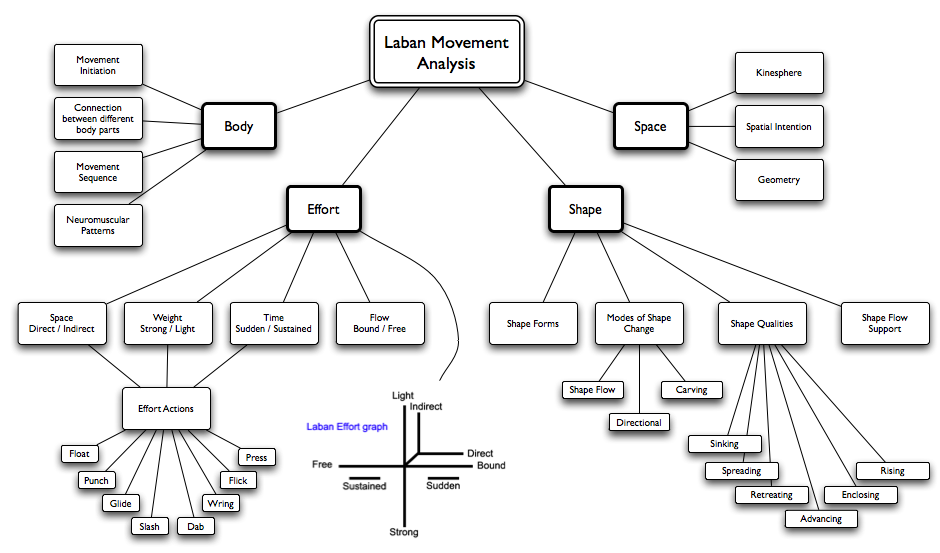
\includegraphics[width=\textwidth]{laban.png}
%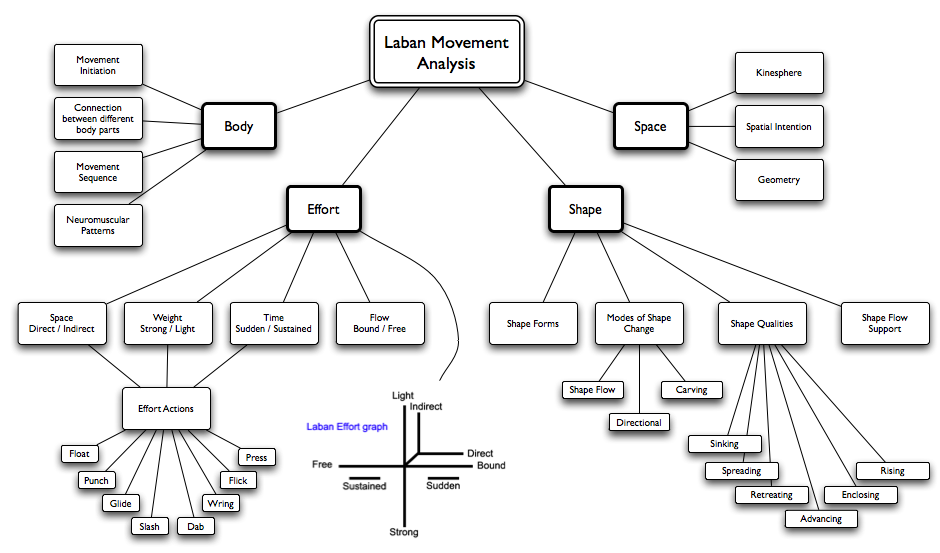
\includegraphics[width=15cm,height=10cm]{laban.png}

\label{labanTree}
\end{figure*}

\mbox{}
\par
There are numerous applications for computerized identification of
the possible qualities that combine to characterize each human
movement. Examples include the generation and control of specific
expressive movements of avatars, virtual characters, or robots in
mixed reality scenarios \cite{Masuda}; understanding of personality traits during a job interview \cite{levy2003use}; severity assessment or revealing of early stages of various disorders such as Alzheimer's, autism, Parkinson's dis-ease \cite{camurri2003application}, or schizophrenia, based on analysis
of a person's motor behavior. Automated emotion recognition from
movement is another important application which may have a
variety of uses such as online feedback to presenters to
help them convey through their body language
the emotional message they want to
communicate (e.g., politicians and public
speakers or actors in training) \cite{nguyen2012online}; as a type of biofeedback for motor skills learning for interpersonal communication,
coordination and self-regulation or recognition of people's emotions during interactive games such as those
played using the Xbox \cite{Zacharatos}.
\mbox{}\\
\par
Several attempts were made to recognize Laban qualities. The first was Chi
et al. \cite{chi2000emote}, who quantified \textit{Effort} and \textit{Shape} for animation.
Most of the other attempts were for emotion recognition in the context of Human Robot Interaction (HRI).
Masuda et al. generated emotional body motion for a humanoid \cite{Masuda}.
Rett et al. proposed a human motion recognition system using a Bayesian reasoning framework \cite{Rett}.
The second line of work focused on LMA and emotions, but not using Kinect.
Lourens et al. \cite{lourens2010communicating} used video data and Samadani et al.
\cite{samadani2013laban} used a high quality MOCAP camera, but both of them
analyzed only hand gestures, rather than whole body movement, which is important for detecting the expression of emotions. A third line of inquiry used Kinect as the main sensor for skeletal information. Gabel et al. \cite{gabel2012full} used Kinect for gait analysis. 
The work of Zacharatos et al. [26] focused on two LMA Efforts (Space Effort and Time Effort) for emotion recognition using Kinect. His feature extraction method was influenced by LMA principles, but he did not attempt to recognize the qualities themselves, and the detection of more than 2 LMA elements are needed to identify expression.
\cite{kim} did attempt to do so but not on a real dataset and their work did not include a performance evaluation. Our work continues Bernstein's et al. work \cite{ran}, but with multitask instead of single-task learning and with analysis on people that are not trained in LMA.
\mbox{}\\
\par
The multi-task learning approach was chosen to address the limitations of the studies cited above. Our goal is to create a method for automated identification of Laban qualities that
characterize any movement sequence, using Kinect.
Our problem presents three challenges. The first is
quantifying subtle qualities for which a well-defined quantification has not yet been found.
The second challenge is handling noisy sensory data with an in-home setup, and the
third is keeping our method as general as possible --- We are developing a system capable of
handling different scenarios (dancing and acting, for example), and different postures (sitting and standing, for example), by different people of different backgrounds (if any)
in movement. For reducing our data collection and analysis effort, we focused our work on 18 Laban qualities
(as listed in table \ref{mixedSummary}) that have been found predictive for emotional state \cite{Tsachor}.

\section{Method}
\subsection{Kinect Sensor Data}
Figure \ref{skeleton} shows the skeleton provided by Kinect's Software Development Kit (SDK).
\begin{figure}[h]
\centering
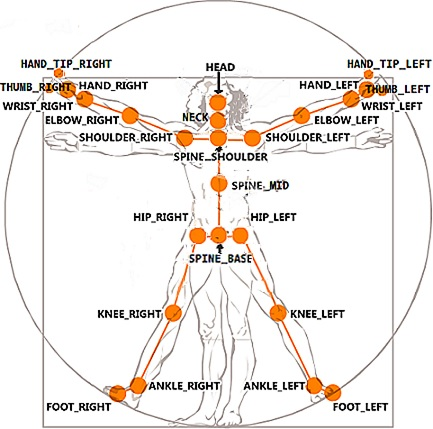
\includegraphics[width=60mm]{skeleton.jpg}
\caption{Skeleton positions relative to the human body}
\label{skeleton}
\end{figure}
Once the skeleton is detected, the 3D coordinates of all the joints of the
user's body --- with the exception of joints that are not visible (e.g., a user's
hand is behind his or her back) --- are provided.
As seen in Figure \ref{Coordinate}, the coordinates are in a ``real-world''
coordinate system, whose origin [0,0,0] is in the sensor and whose x-, y-, and
z-axis are as depicted below.
\begin{figure}[h]
\centering
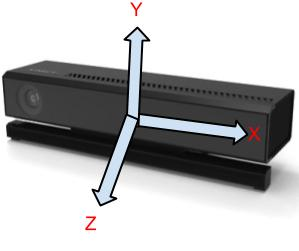
\includegraphics[width=60mm, height=35mm]{KinectV2CoordinateSystem.jpg}
\caption{Kinect Coordinate System}
\label{Coordinate}
\end{figure}

\subsection{Motion Capture Clip Collection}
In order to develop the ability to automatically identifiy Laban qualities that characterize any movement sequence, we generated two specific datasets:
\begin{itemize}
  \item
  The first relied upon Certified Movement Analysts (CMAs) experts in demonstrating the LMA elements. Six CMAs performed 3 second movements of 2-4 LMA elements per clips, generating about 80 clips each, for a total of 550 clips.  Each clip is about 3 seconds long, and the CMAs executed combinations of the 18 qualities.
  To achieve uniform distribution of the Laban qualities over the dataset, in every
  clip a single CMA was asked to perform actions that include several specific qualities,
  and nothing but them.
  
  \begin{figure}[h]
\centering
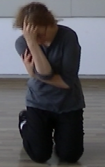
\includegraphics[width=30mm]{Rachelle.png}
\caption{CMA during a clip}
\label{Rachelle}
\end{figure}

\item
Non-CMA dataset - includes 5 subjects that are not CMAs, performing 30 clips each. 
These clips are also about 3 seconds long, and each individual was asked to perform one out 
of several every day tasks.
\end{itemize}
\subsection{Clip Labeling}
To achieve a ground truth labeling for the two datasets, a sample of the first data set clips was tagged by a committee of 2 CMAs (two of the 6 CMAs who performed in the clips) who determined which Laban qualities appear in the clip. The use of a committee decision instead of the subjective opinion of one CMA decreases the labeling noise and the decision is considered as ground truth. The consensus method that the committee used is was: Both of the CMAs watched observed each sample clip without knowing the clip's intended features, named the primary elements observed in the clip independently, then the clip was labeled by the intersection of the two sets where we both agreed. 
\subsection{Feature Extraction}
The feature extraction is adopted from an earlier work \cite{ran}.
Due to the unequal length of clips, all the extracted features are in whole clip 
granularity. We extracted two groups of features, the first is relatively
small, and contains about 100 features each of which is designed for a specific quality. The second group contains about 6000
features, and exploits the rich data that is provided by Kinect, by extracting from every joint in the skeleton, the angular velocity (the change in position of a limb around the fixed point of its joint attachment, e.g, velocity of the limb perpendicular to the radius of the circular motion), acceleration (the change in velocity), and jerk (the change in acceleration). For every joint/metric pair, the mean (average),
variance (how spread the numbers are), skew (how asymmetrical the trajectory appears compared to a bell curve), and kurtosis (how peaked is the trajectory) were extracted (the extraction of the last four
moments is denoted as $\phi$). 



\\\\We denote $\vec{P}_{j}(t)$ as the vector (as we get it from the Kinect) of
the position of joint $j$ in time $t$ in a clip with $n$ frames, and
$\alpha_{j}$ is a coefficient proportional to the mass around the joint. 

\subsubsection{Advance and Retreat}
The Center of Mass (CM) was approximated in this case by the average of all the joints. 
The front of the body was approximated by the perpendicular vector to the vector 
between the Left Shoulder (LS) and the Right Shoulder (RS).
\\\\If $sag$ stands for sagittal, then from the definition of CM of a physical
system,
\begin{equation*}
\vec{P}_{CM}(t) = \sum_{j \in Joints} \alpha_{j}\vec{P}_{j}(t),
\end{equation*}
\begin{equation*}
\vec{P}_{shoulders}(t)=\vec{P}_{LS}(t)-\vec{P}_{RS}(t),
\end{equation*}
the front is perpendicular to $\vec{P}_{shoulders}$, so we can easily calculate it with:
\begin{equation*}
\[\vec{P}_{front}=\vec{P}_{shoulders}\left( \begin{array}{ccc}
0 & 0 & 1 \\
0 & 1 & 0 \\
-1 & 0 & 0 \end{array} \right),\]
\end{equation*}
\begin{equation*}
S_{sag}(t) = \vec{P}_{CM}(t)\cdot\vec{P}_{front}(t),
\end{equation*}
\begin{equation*}
\vec{F}_{sag} = \phi([S_{sag}(1), \ldots S_{sag}(n)]).
\end{equation*}

\subsubsection{Spreading and Enclosing}
This distinction was quantified by measuring the average distance between every joint to 
the vertical axis of the body that extends from the Head (H) to the Spine Base (SB).
\begin{equation*}
d_{j} = \frac{\left|(\vec{P}_{j}-\vec{P}_{SB})\times
(\vec{P}_{j}-\vec{P}_{H})\right|}{\left|\vec{P}_{H}-\vec{P}_{SB}\right|},
\end{equation*}
\begin{equation*}
S_{horiz}(t) = \sum_{j \in Joints} d_{j}(t),
\end{equation*}
\begin{equation*}
\vec{F}_{horiz} = \phi([S_{horiz}(1), \ldots S_{horiz}(n)]).
\end{equation*}

\subsubsection{Rise and Sink}
This distinction was quantified by measuring the average distance on 
axis y of each joint from the CM. This quantification is based on the 
assumption that the body is ``longer'' when rising.
\begin{equation*}
S_{vert}(t) = \sum_{j \in Joints}\left|\vec{P}_{j}-\vec{P}_{CM}\right|,
\end{equation*}
\begin{equation*}
\vec{F}_{vert} = \phi([S_{vert}(1), \ldots S_{vert}(n)]),
\end{equation*}

\subsubsection{Sudden and Sustained}
This distinction was quantified by the skew of the acceleration, relying on the assumption that the acceleration of a sudden movement will be skewed further to the left, i.e., will get a higher value at the beginning of the movement.
\begin{equation*}
\vec{V}_{j}(t) = \vec{P}_{j}(t+1) - \vec{P}_{j}(t),
\end{equation*}
\begin{equation*}
\vec{a}_j(t) = \vec{V}_{j}(t+1) - \vec{V}_{j}(t),
\end{equation*}
\begin{equation*}
Skew_j = \frac{1}{n}\sum_{i=1}^{n}(\frac{a_j(t) - \mu}{\sigma})^3
\end{equation*}
where $\mu$ and $\sigma$ are the mean and standard deviation of the accelerations ($a_j(t)$), and n is the length of the the time series (clip).
\subsubsection{Direct and Indirect}
In Direct movement, the distal limb part is likely to have a straight trajectory, and the mid-limb parts will have a slightly different vector and perhaps have a different direction.  In Indirect movement, the proximal part of the limb will likely move much less than the distal part of the limb on a curve.   Directness may also be expressed in the gaze, which we did not measure. We quantified how straight is the trajectory by the angle between the movement vector of a joint to the one that is created by the next frame in the clip (in a direct movement the angle between them is small).
The velocity direction $V$ is calculated by
\begin{equation*}
\vec{V}_{j}(t) = \vec{P}_{j}(t+1) - \vec{P}_{j}(t),
\end{equation*}
and the angles between a direction to the next one is calculated with the inner product
\begin{equation*}
\vec{A}_{j}(t) = \vec{V}_{j}(t+1) \cdot \vec{V}_{j}(t).
\end{equation*}

\subsubsection{Jump}
This distinction was quantified by the maximal (over the clip) difference in the position along the Y axis of the lower between Ankle Right (AR) and Ankle Left (AL). 
\\Let $S(t)$ be the time series of the minimum between the ankles.
If $P_{j}^{Y}(t)$ is the position along Y axis of joint j in time t,
\begin{equation*}
S(t) = min\{P_{j}^{Y}(t), P_{j}^{Y}(t)\},
\end{equation*}
\begin{equation*}
F_{Jump} = max_{t}\{S(t)\} - min_t\{S(t)\}.
\end{equation*}
i.e., the highest point of the bottom of the skeleton minus the lowest point of the bottom of the skeleton.

\subsubsection{Statistical glance on the features}
Examples of qualities and their most significant feature are given in 
Table \ref{bestFeatures}. The ``Information Gain'' metric used
in the table is defined as:
\begin{equation*}
       IG(T,f) = H(T) - H(T|f),
\end{equation*}
where T is the training set, f is a feature, and H() is the information
entropy of a dataset.
\begin{table*}
   \centering
   \caption{Example of several qualities and the feature found to be
   the most informative for them. ``Relative position'' stands for the
   position of the joint relative to the ancestor joint in the joint
   hierarchy.}
   \csvautotabular{rankFeatures.csv}
   \label{bestFeatures}
\end{table*}

\subsection{Multilabel Classification using Multitask Learning}
 

Multi-task learning was chosen as particularly suited to address challenge 3:  Developing a system capable of identifying movement in different scenarios, different postures by people of different movement backgrounds. Multilabel learning is suited to this task because it deals with problems where each instance is associated with multiple labels simultaneously, where the number of labels is not fixed from instance to instance. 

The task of this learning paradigm is to predict
the label (Laban quality) set for each unseen instance (skeletal recording), 
by analyzing training instances with known label sets. The multilabel
approach taken in this paper is to break the LMA problem into 18
binary classification tasks --- one for every Laban quality --- where every binary
decision is whether or not the quality exists. 
In this paper we chose to tackle Multilabel Classification problem using
Multi-task learning (MTL) and we showed how it outperforms the more common
Single Task Learning (STL).
MTL framework \cite{caruana1997multitask} is an approach to ML that learns a problem simultaneously with other related problems at the same time, using a shared representation, even when they are different. This differs from STL, which trains a model for every task separately, and the data might be represented for each one differently.
The goal of MTL is to improve the performance of learning algorithms by learning classifiers for multiple tasks jointly. This works particularly well when these tasks have some commonality and are generally slightly under sampled.
For the multitask setup we used Multitask Elastic Net (MEN) regularization, which is the multitask regularization method of Zou et al. \cite{Zou}, where the optimization objective is:
\\
\begin{equation}\label{eq:MEN}
\|Y - XW\|^2_F+\lambda_1\cdot\|W\|_{2,1}+\lambda_2\cdot\|W\|^2_F,
\end{equation}

$\lambda_1$, and $\lambda_2$ are hyper-parameters, where,
\\
\begin{equation*}
\|W\|_{2,1} = \sum_i \sqrt{\sum_j w_{ij}^2},
\end{equation*}
i.e., the sum of norm of each row (also known as mixed norm), and
\begin{equation*}
\|W\|^2_F = \sum_i{\sum_j w_{ij}^2},
\end{equation*}
i.e., the Frobenius norm.
Feature selection was carried out by averaging the statistical significance of
each feature with respect to all of the tasks (this is in contrast to the single
task learning flow, where every task had its own feature selection). As seen in
Table \ref{MultitaskVsSeparated}, the multitask setting improved the F1 score (will be explained below) by 4\% over the STL results, indicating that the tasks are correlated and more might be learned from the small dataset when using this setting.
\subsection{Performance Evaluation}
From a statistical point of view, we have 18 possible labels (Laban qualities) for every clip. 
Each clip was a combination of just a few of these, often 3-4, which means that there is about 
an 85\% chance that a quality won't appear in a clip. Due to this sparsity,
accuracy (the number of clips that have been labeled correctly out of the
total number of clips) alone is not a relevant metric for the performance
evaluation because one can get 85\% accuracy by stating that for every recording none of the qualities appear.
From one Laban quality point of view, let Truly Positive Clips (TPC) stand for clips that the quality truly appears in them, and let Classified Positively Clips (CPC) stand for clips that our classifier found that include the quality. A better evaluation would have to combine the precision (the fraction of retrieved clips that were relevant) and recall (the fraction of relevant instances that were retrieved) rates of the
classifier, where
\begin{equation*}
precision = \frac{|\{TPC\}\cap\{CPC\}|}{|\{CPC\}|}.
\end{equation*}
\begin{equation*}
recall = \frac{|\{TPC\}\cap\{CPC\}|}{|\{TPC\}|}.
\end{equation*}
 The combination between the two can be done using the F1 score:
\begin{equation*}
F_{1} = \frac{2\cdot precision\cdot recall}{precision+recall}.
\end{equation*}
The F1 score was chosen as the main evaluation metric in this paper.
\section{Experimental Setups and Results}

\subsection{Multitask vs Single Task Learning}
We found that multitask learning for all the 18 qualities together exhibited superior
performance to learning a classifier for each problem separately.
\begin{table}[ht]
\centering
\begin{tabular}{|p{1.8cm}|p{1.8cm}|p{1.8cm}|}
\hline
Metric&Single task&Multitask\\\hline
Precision&0.46&\textbf{0.59}\\\hline
Recall&\textbf{0.71}&0.65\\\hline
F1&0.56&\textbf{0.6}\\\hline
\end{tabular}
\caption{Multitask vs Single task learning performance evaluation on a data set of several CMA's.}
\label{MultitaskVsSeparated}
\end{table}

\subsection{Evaluation of Performance by Laban Quality}
The performance over every quality as classified by the MEN in Table
\ref{mixedSummary}. During the MEN optimization ~\eqref{eq:MEN}, the mixed norm
term $\|W\|_{2,1}$  promotes sparsity in the weights matrix $W$ such that for
every row in the matrix, if one coordinate is equal to zero, then every coordinate
in the row will be equal to zero.
\\The generalization ability of the model was enhanced by the fact that the
decision which features to select is influenced by all the qualities, (feature $f_i$ is
selected in the MEN if the row $r_i$ in $W$ is not all zeros). The most
significant improvement were in the qualities that performed worse in the
single task learning setting (\textit{Strong} and \textit{Sudden} for example).
\begin{table}[!h]
\centering
\begin{tabular}{|p{3cm}|p{0.9cm}|p{0.9cm}|p{0.9cm}|}
\hline
Quality&Precis-ion&Recall&F1 score\\\hline
Jump&0.89&0.81&0.85\\\hline
Twist and Back&0.69&0.85&0.76\\\hline
Sink&0.62&0.79&0.69\\\hline
Rhythmicity&0.59&0.72&0.65\\\hline
Spread&0.55&0.76&0.64\\\hline
Head drop&0.60&0.66&0.63\\\hline
Rotation&0.66&0.60&0.63\\\hline
Free and Light&0.45&0.94&0.61\\\hline
Up and Rise&0.67&0.54&0.60\\\hline
Condense and Enclose&0.44&0.84&0.58\\\hline
Arms To Upper Body&0.67&0.54&0.60\\\hline
Advance&1.00&0.38&0.55\\\hline
Retreat&0.50&0.59&0.54\\\hline
Passive&0.40&0.85&0.54\\\hline
Bind&0.44&0.61&0.51\\\hline
Direct&0.56&0.49&0.52\\\hline
Sudden&0.61&0.41&0.49\\\hline
Strong&0.29&0.42&0.34\\\hline
\textbf{Average}&\textbf{0.59}&\textbf{0.65}&\textbf{0.60}\\\hline
\textbf{SD}&\textbf{0.17}&\textbf{0.17}&\textbf{0.11}\\\hline
\end{tabular}
\caption{Recall, precision and F1 score of each Laban quality on a CMA
mixture dataset. The learning was done in a multitask setting. The number of
features that weren't nullified by the mixed norm regularization is
282 (same features for all of the tasks). The F1 average and standard
deviation over the qualities is shown in the last row of the table.}
\label{mixedSummary}
\end{table}

\subsection{Evaluation on an Unseen CMA}
In this experiment the test set was taken from a CMA who did not appear in the train set.
As shown in Figure \ref{domainAdaptationBaseLine}, performance degrades on the unseen CMA from 0.6 to 0.57.
This degradation seems minimal for such a large variability between clips from one CMA to another. Every CMA performed different gestures, in different postures (some sitting and some standing) 
and in different contexts (some were dancing while some were acting).

\begin{figure}[!h]
\centering
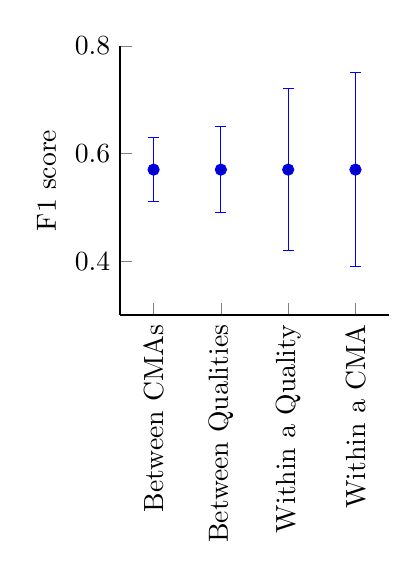
\begin{tikzpicture},
\centering
\begin{axis}[
height=5cm,
width=5cm,
ylabel={F1 score},
ymax=0.8,
ymin=0.3,
xmin=0.5,
xmax=4.5,
axis y line*=left,
axis x line*=bottom,
xticklabels={Between CMAs, Between Qualities, Within a Quality, Within a CMA},
xtick={1,2,3,4},
x tick label style={rotate=90,anchor=east}]
\addplot+[only marks][error bars/.cd,y dir=both, y explicit]
coordinates {
(1,0.57) +- (0.06,0.-0.06)
(2,0.57) +- (0.08,0.08)
(3,0.57) +- (0.15,-0.15)
(4,0.57) +- (0.18,-0.18)
};
\addplot[dashed] coordinates {(0,0) (10.5,0)};
\end{axis}
\end{tikzpicture}
\caption{Confidence intervals of F1 score in quality detection of an unseen CMA.
Every confidence interval is two standard deviations (STD) long.
In every trial one CMA was the test set, while the classifier was trained on the rest. The mean F1 score is 0.57. The measures from left to right are: STD between CMAs when every CMA's score is an average the scores of his or her qualities; STD between qualities when every quality's score is an average of all of the CMAs' scores for this quality; an average of qualities' STDs, where every STD is between CMAs within a quality; an average of CMAs' STDs, where every STD is between qualities within a CMA's dataset.}
\label{domainAdaptationBaseLine}
\end{figure}

\subsection{Validation on Untrained Movers in Everyday Tasks}
The final validation was conducted on ordinary people (non-CMAs). We
designed several daily actions (greeting friends or playing with a balloon, for
example) and the CMA committee tagged the clips. This dataset was small, with a
focus on the qualities that we found easier to recognize. The evaluation is shown in Figure \ref{nonCMAs}.

\begin{figure}[ht!]
\centering
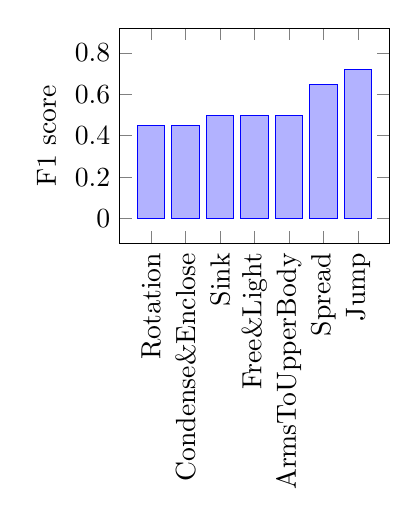
\begin{tikzpicture}
\begin{axis}[
ymin=0,
ymax=0.8,
width=5cm,
ybar stacked,
enlargelimits=0.15,
ylabel={F1 score},
symbolic x coords={Rotation,Condense\&Enclose,Sink,Free\&Light,ArmsToUpperBody,Spread,Jump},
xtick=data,
x tick label style={rotate=90,anchor=east},
]
\addplot+[ybar] plot coordinates  {(Rotation,0.45) (Condense\&Enclose,0.45) (Sink,0.5)
(Free\&Light,0.5) (ArmsToUpperBody,0.5) (Spread, 0.65) (Jump,0.72)};

\end{axis}
\end{tikzpicture}
\caption{Performance on ordinary people (non-CMAs) instructed to
perform several tasks.}
\label{nonCMAs}
\end{figure}

\section{Discussion}
The authors of this study generated video clips of 18 LMA elements found to be significant in the expression of emotion, in combinations found together in the expression of particular emotions in other studies[23].  The unique data set generated of these particular LMA elements focused our ML priorities to automatically identify the specific LMA elements most helpful to therapeutic, communication and gaming applications.   Using CMA's as expert movers for these data sets and filtering the training set a second time with trained CMA observers boosted the accuracy of the training set.   Filtering the test set in this way by tagging all clips (rather than the sample tagging within the scope of this study) may further boost  accuracy when tested in non-structured settings.      

An advantage of the language of LMA is that it can be more easily understood as language  than metric descriptions, describes in words that can be used for coaching, and facilitates first-person embodied experience of movement. Thus automatic recognition that uses this language can be readily applied in scientific, artistic, and humanistic practices.

Although not within the scope of this paper, the specific results of the feature extraction itself may also be valuable in better understanding the kinesiologic mechanisms by which qualitative movement is recorded and perhaps produced in the body.   The precision and recall themselves may illuminate nuances in movement vectors, relationships among body parts, and how these change over time that open new inquiry into each LMA element itself. 

While automatic recognition of Body, Space and somewhat for Shape is easier to achieve than recognition for Effort, the recall and F1 score for some Efforts (notably the combination of Free and Light) are quite high.  The Efforts which we're not yet identifying clearly (such as Strong, or Direct) more interdisciplinary led exploration may yield new analytical hypotheses for analysis from the same data set --- for example,  Identification of Direct might be improved by looking at vectors for the distal limb parts compared to vectors for the mid-limb and proximal parts. 

We discovered advantages for multi-task learning in identifying some elements, and advantages for single task for others. STL had advantages for recall, and multi-task for precision. This indicates a future development of these methods might combine each as a filter to boost accuracy further still.

\section{Conclusion}
The improvement of the F1 score from a single task learning setting (0.56) to a multitask setting (0.6) demonstrates the synergy of a shared model for several correlated tasks. 
The method works better on qualities that appear with larger changes in \textit{Space} that supports their recognition. 
Although this fact indicates that there still much more to be done to achieve a deep capture of all the qualities, the MTL approach might facilitate the ML to take advantage of LMA theories of the affinity of space, shape, effort and body to mine the data for new discoveries about the kinematic features of effort.  
The high performance on free and light demonstrated that this method can identify some Efforts and shows potential that with further refinement it maybe valuable for recognition of the other Efforts. 
We defined  three challenges in the introduction: the first, quantifying the subtle qualities --- 
the MTL approach produced modest improvement in that area.
The second, handling noisy sensory data --- We used multiple signal processing and ML manipulations to extract meaningful features from raw skeletal recordings, and were able to produce semantic knowledge from the data. 
The third, developing a method capable  of generalization from novel and varied input data, was the strongest achievement of our method. Our method succeeded with a first time seen CMA and with ordinary people in several postures doing different tasks. 
The mild degradation of the F1 score from a seen CMA (0.6) to an unseen (0.57) shows the generalization ability is robust.
This generalization ability is derived from our focus on the MEN regularization terms, which kept our model to not be too-rich, even sparse, and thus not over-fitted on the training data.
In summary, we succeeded in capturing the essence of many LMA qualities, in non-laboratory settings, demonstrating that it is possible to develop an in-home, inexpensive LMA based feedback system for multiple purposes such as therapy, arts, communication, HRI and inter-cultural understanding of movement.
\bibliographystyle{unsrt}
\bibliography{bib}

\end{document}
